\documentclass{article}

\usepackage[utf8]{inputenc}
\usepackage{graphicx}
\usepackage[brazil]{babel}
\usepackage[utf8]{inputenc}
\usepackage{amsthm,amsfonts,amssymb}
\usepackage{enumitem}
\usepackage{tabularx}
\usepackage{siunitx}

\usepackage{ragged2e}
\usepackage{times}
\usepackage{microtype}

\baselineskip 65 mm

\begin{document}

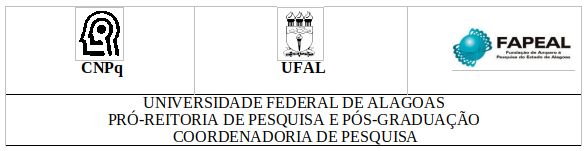
\includegraphics[width=1.0\columnwidth]{tabela1.png}

\begin{center}
PROGRAMA INSTITUCIONAL DE BOLSAS DE INICIAÇÃO CIENTÍFICA
PIBIC/UFAL/FAPEAL/CNPq

\vspace{7mm}
\textbf{RELATÓRIO PARCIAL (2018– 2019)}
\end{center}
   
\vspace{6mm}
   
\begin{flushleft}
\textbf{TÍTULO DO PROJETO DE PESQUISA:}
\underline{Aplicações Inovadoras da Teoria da Informação no Processamento e Análise de Imagens e Sinais}
\vspace{5mm}


\textbf{TÍTULO DO PLANO DE TRABALHO:}
\underline{Análise de Séries Temporais com Teoria da Informação}
\vspace{5mm}
    
\begin{table}[!h]
\begin{center}
\begin{tabularx}{\textwidth}{|X|X|X|}
\hline                              
\textbf{Nome Orientador/Unidade/Campus/Email} &  Alejandro César Frery Orgambide / Universidade Federal de Alagoas / Campus A.C. Simões / acfrery@ic.ufal.br\\
\hline     
\textbf{Nome Bolsista ou Colaborador} & Roger de Almeida Matos Junior\\
\hline     
\textbf{Email/Fones} & ramj@laccan.ufal.br / (82)98717-2878\\
\hline     
\end{tabularx}
\end{center}
\end{table}
\end{flushleft}
    
\begin{center}
\begin{tabular}{|c|c|c|c|}
\hline
X & Bolsista CNPq & & Bolsista FAPEAL\\
\hline
 & Bolsista UFAL & & Colaborador\\
\hline
 & Bolsista CnPq-Af & & \\
\hline
\end{tabular}
\end{center}
  
\newpage
\begin{center}
\textbf{\large{RESUMO}}

\hrulefill

\end{center}

É relatado aqui o processo de aperfeiçoamento de algoritmos de técnicas de imputação de dados que lidam com os padrões não observados pela metodologia de Bandt \& Pompe \cite{bandt2002permutation}. Os algoritmos foram feitos na linguagem de programação C por esta ser mais veloz e tão precisa quanto o R. Após discutir sobre os objetivos deste projeto, esse trabalho apresenta as etapas do desenvolvimento de tais algoritmos e os resultados com eles alcançados.


\textbf{Palavras-chave:} Séries Temporais, Teoria da Informação, Imputação de dados, Interface \textit{.Call()}.
 
\newpage
\begin{center}
\textbf{\large{OBJETIVOS DO PROJETO DE PESQUISA}}\\
\hrulefill \\
\end{center}
          
O objetivo geral deste projeto é avançar na fronteira do conhecimento sobre séries temporais, obedecendo diretrizes não-paramétricas e utilizando a Teoria da Informação.
Almejamos desenvolver uma plataforma unificada de análise de séries temporais com métodos de simbolização. Daremos ênfase ao problema da imputação de padrões ausentes, tendo as seguintes metas em vista: estudar e implementar técnicas para imputação de padrões ausentes ocasionados por dados repetidos; analisar a capacidade de reconstrução de informações dessas técnicas quando a série temporal é armazenada com menos precisão do que a ideal; analisar a distribuição temporal dos padrões originais e imputados; desenvolver uma ferramenta para análise de séries temporais baseada em padrões ordinais utilizando a linguagem R.
    
\newpage
\begin{center}
\textbf{\large{OBJETIVO ESPECÍFICO DO TRABALHO DO ALUNO}}

\hrulefill 

\end{center}
    
Desenvolver técnicas de imputação de padrões não observados pela metodologia de Bandt \& Pompe. Avaliar a capacidade dessas técnicas de resistir à perda de precisão dos dados observados. Integrar as técnicas em um sistema de produção de análise de séries temporais desenvolvido na plataforma R.
    
\newpage
\begin{center}
\textbf{\large{ETAPAS DO PLANO DE TRABALHO INDIVIDUAL DO ALUNO}}

\hrulefill 

\end{center}

\begin{flushleft}    
\textbf{Conhecer a fundo a técnica de análise de séries temporais de Bandt \& Pompe, suas limitações, possíveis implementações e aplicações.}
\end{flushleft}

O estudo de artigos sobre a técnica de análise de séries temporais de Bandt \& Pompe foi realizado a fim de uma familiarização com o tema, para que se pudesse compreender seu funcionamento e depois implementá-lo.
Com isso, foram estudados tópicos como séries temporais e sua simbolização através de padrões ordinais gerados a partir do método de Bandt e Pompe, técnicas de imputação de padrões ausentes e descritores como entropia, complexidade estatística e distância estocástica.


\begin{flushleft}
\textbf{Aprender o uso da plataforma R}
\end{flushleft}


A linguagem R foi escolhida por se tratar de uma linguagem matemática muito conveniente para a realização de cálculos estatísticos. Ao longo desse período foi feito um estudo online sobre o funcionamento dessa linguagem, seguido pela prática a fim de estabelecer um maior aprendizado sobre a mesma.\\


\begin{flushleft}
\textbf{Desenvolver protótipos de algoritmos de imputação de padrões não observados}
\end{flushleft}


O desenvolvimento de algoritmos eficientes para a imputação de padrões ausentes ocasionados por dados repetidos foi a parte principal no desenvolvimento do projeto ao longo desse período. 
Os algoritmos para imputação desses padrões já haviam sido implementados na plataforma R anteriormente. Contudo, em busca de maior velocidade no tempo de execução desses algoritmos foi encontrada uma possível solução através da interface \verb|.Call()|~\cite{Speed}, que pode chamar funções em C dentro de um programa em R, e por C ser uma linguagem de baixo nível, sua velocidade de execução é muito maior, logo era uma opção viável para chegar ao objetivo desejado.
Com isso, foi estudado o funcionamento desta interface, suas aplicações, e então as funções para imputação desses padrões começaram a ser implementadas em C dentro do formato requerido por essa interface.


\newpage
\begin{center}
\textbf{\large{APRESENTAÇÃO E DISCUSSÃO DOS PRINCIPAIS RESULTADOS OBTIDOS DURANTE O PRIMEIRO SEMESTRE DA PESQUISA}}

\hrulefill 

\end{center}
    
Por ser uma linguagem voltada à matemática, R é uma das linguagens de programação mais convenientes para se realizar cálculos estatísticos. Contudo, para um número muito alto de dados de entrada, o R pode se mostrar consideravelmente lento.


Os algoritmos em R anteriormente criados para a imputação de padrões de séries temporais se mostraram eficazes e precisos em seus resultados. Porém, tendo em vista que era necessária a análise de séries temporais de tamanho muito grande, os algoritmos possuíam um tempo de execução muito alto. Com isso veio a necessidade de um meio de incrementar a velocidade desses algoritmos.

Por outro lado, C é uma linguagem de programação que possui recursos de baixo nível, e é conhecida por sua eficiência, velocidade e portabilidade. Assim, uma solução encontrada para o problema da velocidade foi a utilização da interface \verb|.Call()|, que funciona como uma ponte entre as duas linguagens, possibilitando “chamar” funções escritas em C dentro de um código em R, e assim transmitindo dados entre as duas plataformas.

Em seu modelo proposto, Bandt e Pompe assumiram que os dados seriam valores contínuos, ou seja, desconsidera que possa haver repetição dos mesmos. Sendo assim, sua simbolização não abrange esses casos, o que provoca a ausência dos padrões que representariam esses dados para que se pudesse ser feita sua distribuição de probabilidade. Com isso, algumas soluções são utilizadas para se resolver esse problema, essas soluções são as técnicas de imputação, são elas a Complete Case, Time Ordered, Random e Data Driven~\cite{traversaro2018bandt}.

Os algoritmos citados são implementações desses quatro métodos. Sua implementação em C foi feita da seguinte forma: a função em C é declarada como retornando um tipo SEXP, que significa Simple EXPression, todos os dados divididos entre as duas linguagens precisam ser deste tipo, ou seja, todos os dados recebidos pela função em C são desta forma e o array de distribuição de probabilidade criado pela função também assume esse tipo. O arquivo .c deve ser compilado com o comando \verb|R CMD SHLIB arquivo.c|, isso gerará um novo arquivo do tipo .so. No sistema em R, esse arquivo .so deve ser carregado através do comando \verb|dyn.load(arquivo.so)|, em seguida se pode utilizar a função em C através da interface utilizada com \verb|.Call(função, ...)|, onde após o nome da função são inseridos todos os parâmetros necessários~\cite{.Call,Extensions}.

Até o presente já foram implementadas dessa forma duas das quatro técnicas de imputação, a Complete Case e a Time Ordered. \\
Para se testar a velocidade e acurácia das versões em C, foram executadas diversas vezes as versões em ambas as linguagens a partir das mesmas entradas, com séries temporais geradas de tamanho igual a trinta mil. Com isso foram obtidas duas distribuições de probabilidade, para testar a acurácia foram calculadas as entropias de cada uma das distribuições separadamente e depois comparadas, era mais conveniente comparar as entropias pois deveriam ser iguais se as distribuições de probabilidade fossem iguais, e por cada uma se tratar de um único valor numérico foi possível utilizar o LRE (\textit{Log-Relative Error})~\cite{almiron2010numerical}, que consiste no seguinte:

$$ LRE(x,c)
= \left\{\begin{array}{rll}
- \log_{10} \frac{|x-c|}{|c|} & \hbox{se} & c \neq 0 \\
- \log_{10} |x| & \hbox{caso contrário}
\end{array}\right.$$

Onde c é o valor verdadeiro e x é o valor a ser comparado, a função nos retornará a quantidade de dígitos significantes que foram corretamente computados. Em cada uma das execuções o resultado obtido foi o seguinte:

    
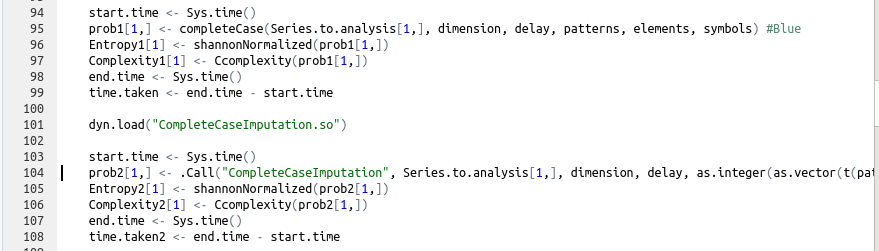
\includegraphics[width=0.80\columnwidth]{LRE.png}


Ou seja, os resultados de ambas as funções são iguais, o que implica que a versão é C é acurada.
Quanto à velocidade, os resultados também se mostraram positivos. Para calcular o tempo de execução de cada uma foi utilizado o seguinte algoritmo:
    
\begin{flushleft}
\textit{start.time $<$- Sys.time()\\
--- função a ser analisada ---\\
end.time $<$- Sys.time()\\
time.taken $<$- end.time - start.time\\}
\end{flushleft}

Onde a variável time.taken nos diz exatamente o tempo levado para executar a função testada.

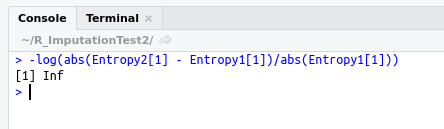
\includegraphics[width=0.80\columnwidth]{Code.png}

Abaixo segue uma tabela, baseada numa amostra obtida a partir de dez distintas execuções dos programas, comparando os tempos de execução das implementações do Complete Case em cada linguagem:\\


\begin{tabular}{|c|c|c|c|}
     \hline
      & Valor mínimo & Valor máximo & Média\\
      \hline
      R & \SI{31.67778}{\second} & \SI{34.97058}{\second} & \SI{33.05312}{\second}\\
      \hline
      C & \SI{0.321858}{\second} & \SI{0.3651605}{\second} & \SI{0.3360521}{\second}\\
      \hline
\end{tabular}\\


Ou seja, tendo como base a média de tempo, é fácil ver que a versão em C é aproximadamente cem vezes mais veloz que a versão em R.
Quanto à implementação da Time Ordered, analisando também sua velocidade em ambas as versões, com o mesmo número de amostragem, obtém-se a seguinte tabela:\\


\begin{tabular}{|c|c|c|c|}
     \hline
      & Valor mínimo & Valor máximo & Média\\
      \hline
      R & \SI{129.3993}{\second} & \SI{142.9892}{\second} & \SI{135.4226}{\second}\\
      \hline
      C & \SI{1.806375}{\second} & \SI{1.903321}{\second} & \SI{1.849567}{\second}\\
      \hline
\end{tabular}\\

Tal qual o Complete Case, vemos que a velocidade da versão em C do Time Ordered supera em muito a versão em R.
Com isto, temos que os algoritmos sendo desenvolvidos em C serão mais vantajosos, pois possuem a mesma precisão mas com superior velocidade, o que facilitará suas aplicações no futuro.

\newpage
\begin{center}
\textbf{\large{CRONOGRAMA DE ATIVIDADES}}

\hrulefill 

\end{center}

\begin{flushleft}    
\textbf{Atividade 1:} Conhecer a fundo a técnica de análise de séries temporais de Bandt \& Pompe, suas limitações, possíveis implementações e aplicações.
\newline
\textbf{Atividade 2:} Aprender o uso da plataforma R.
\newline
\textbf{Atividade 3:} Conhecer técnicas de projeto e implementação de interfaces amigáveis usando R.
\newline
\textbf{Atividade 4:} Desenvolver protótipos de algoritmos de imputação de padrões não observados.
\newline
\textbf{Atividade 5:} Aplicar as técnicas desenvolvidas a conjuntos de dados de propriedades conhecidas.
\newline
\textbf{Atividade 6:} Integrar as técnicas desenvolvidas em uma plataforma de produção.
\end{flushleft}
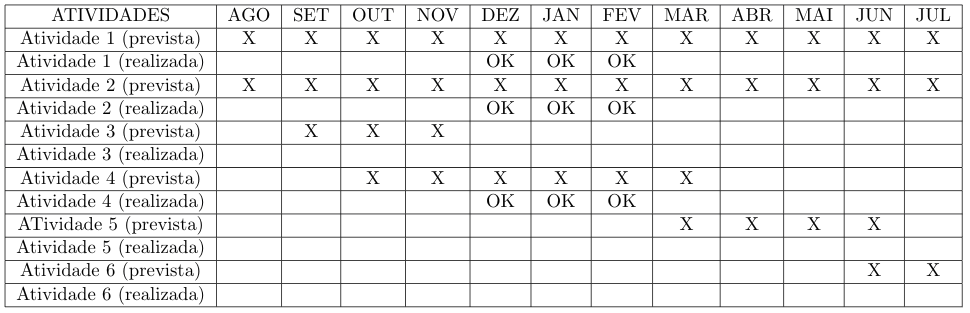
\includegraphics[width=1.1\columnwidth]{tabela}
* As atividade 1, 2, 3 e 4 não foram realizadas antes do mês de dezembro porque neste mês houve uma substituição de bolsista.

\newpage
\begin{center}
\textbf{\large{FATORES POSITIVOS E NEGATIVOS QUE INTERFERIRAM NA CONDUÇÃO DO PROJETO E PLANO DE TRABALHO}}

\hrulefill 

\end{center}
\textbf{Positivos:}
\begin{itemize}
    \item Experiência com pesquisa científica.
    \item A possibilidade de aprender uma nova linguagem de programação(R).
    \item Aprendizagem na área de estatística e na análise não-paramétrica de dados.
\end{itemize}
\textbf{Negativos:}
\begin{itemize}
    \item Dificuldade em encontrar material físico sobre R.
\end{itemize}

\newpage
\bibliographystyle{plain}
\bibliography{referencias.bib}

\end{document}
